% ============================================================
% Appendix A: Schematics and Layouts
% ============================================================
\chapter{Schematics and Layouts}
\label{app:schematics}
% the figures of this appendix are placed here ([H]); pages end where they end
% instead of spreading the space between heading, text and figure
\raggedbottom

This appendix contains photographs of the boards, the schematic of the retrofitted test-diagnosis module and the printed circuit board (PCB) layouts of its four boards, all designed by Leyer~\cite{leyer2023}. The schematic sheets and the layout views were rendered with KiCad from the Eagle design files of 2024, in which this work replaced the displays and split his board design into one file per board. The schematic comes from its Rev~1.0 file, the Upper, LED and \gls{stm32} boards from their Rev~1.0 files, the Base Board from the combined design file, which still labels it Rev~0.0. Schematic sheet~3 and the LED Board are therefore shown with the \texttt{SC03-12EWA} displays (\texttt{DS1}, \texttt{DS2}) listed in \Cref{tab:bom}. The schematic sheets are vector graphics, best read zoomed in on screen; the unit letters after a designator (e.g.\ \texttt{AR} in \texttt{X4AR}) are KiCad's and may differ from the gate names of the Eagle design. Each layout view shows the outer copper layer, the silkscreen and the outline of one side; the inner layers are left out, and the bottom views are mirrored, as seen from below. The German labels are those of the design files. A graphic logo and a board designation of third-party origin have been masked in the photographs, and on the unpopulated Rev~1.0 \gls{stm32} Diagnostics Board also the production code of the PCB manufacturer; the layout views leave out the logo and the designation, both drawn in copper in the design files. No electrical content is affected.


% ------------------------------------------------------------
\section{Board Photographs}
\label{app:rev0_photos}

The first two photographs show boards of the inherited Rev~0.0 prototype, which required the rework and debugging discussed in \Cref{subsec:hardware_challenges}. The other two show unpopulated boards: the Base Board, which was reused in its inherited revision, and the corrected Rev~1.0 \gls{stm32} Diagnostics Board.

\begin{figure}[H]
	\centering
	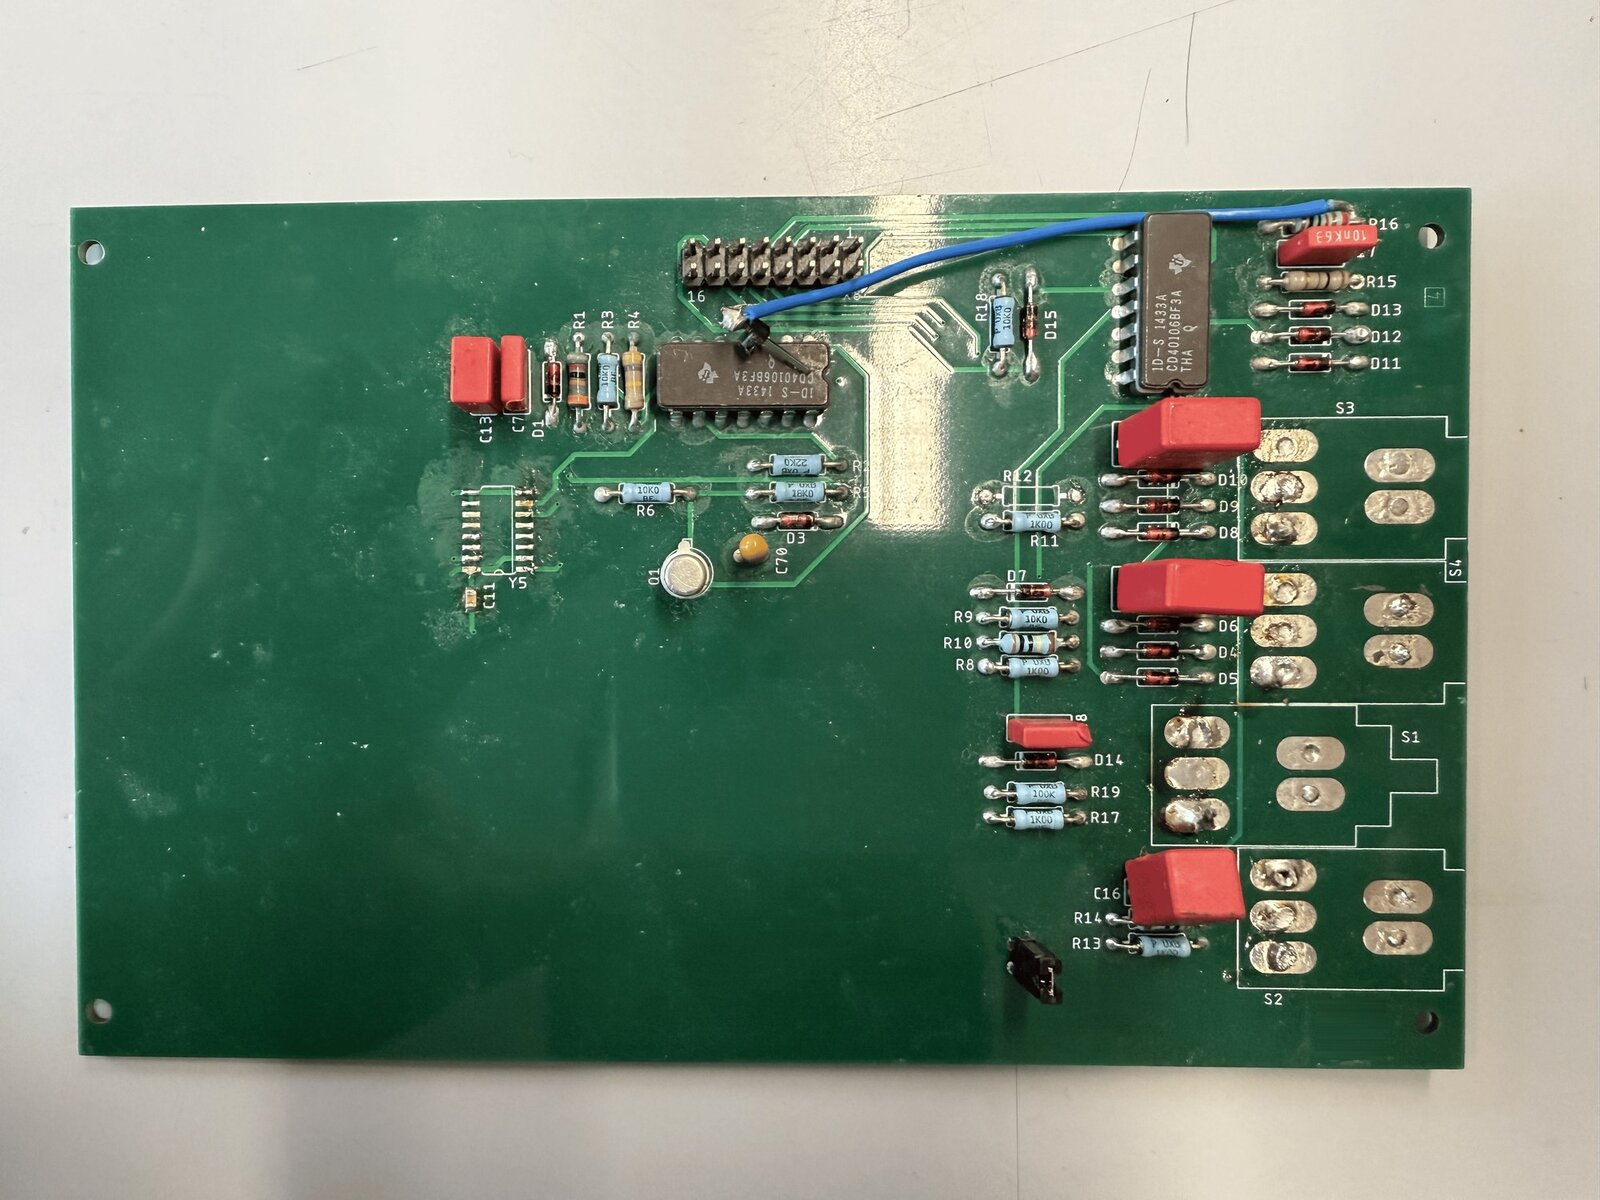
\includegraphics[width=0.75\textwidth]{photos/rev0_upper_board_top.jpg}
	\caption[Rev 0.0 Upper Board]{Inherited Rev~0.0 Upper Board, populated (top view). The blue wire was added to the prototype by hand.}
	\label{fig:rev0_upper_board}
\end{figure}

\begin{figure}[H]
	\centering
	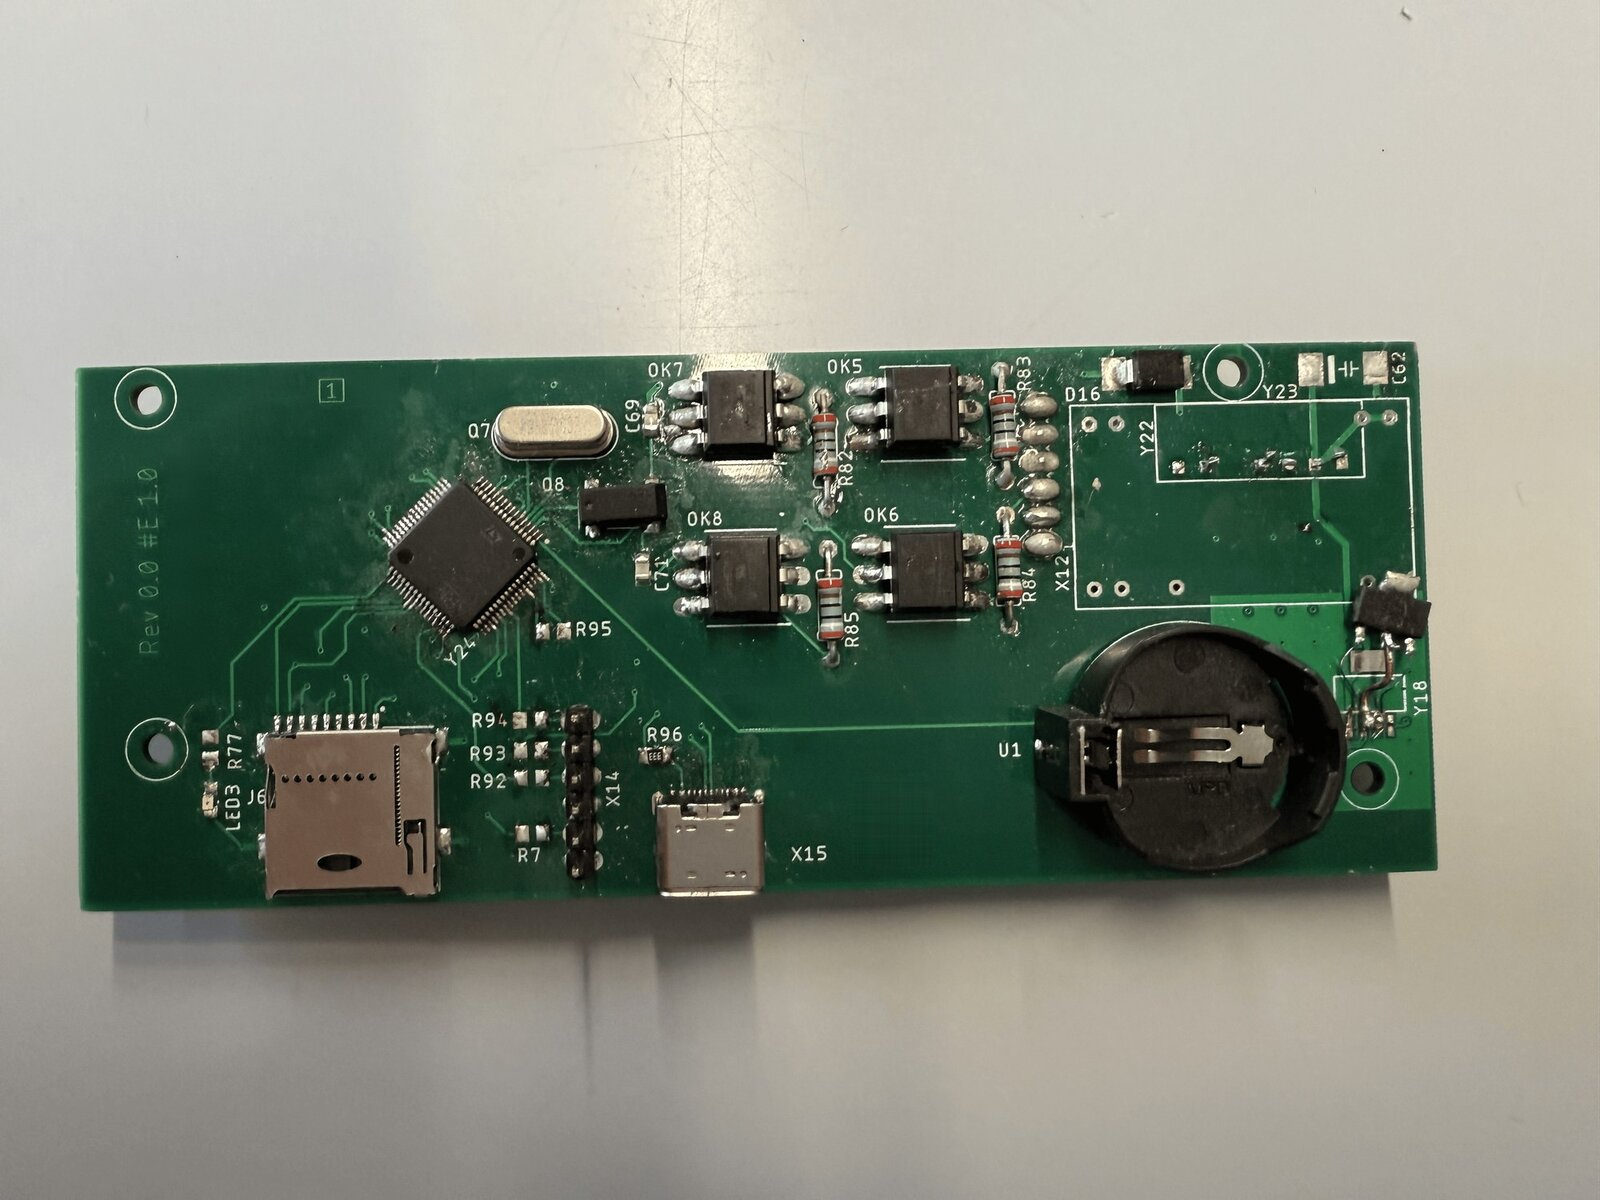
\includegraphics[width=0.75\textwidth]{photos/rev0_stm32_board_top.jpg}
	\caption[Rev 0.0 STM32 Board]{Inherited Rev~0.0 \gls{stm32} Diagnostics Board, populated (top view). Its SWD header \texttt{X14} is wired as on Rev~1.0.}
	\label{fig:rev0_stm32_board}
\end{figure}

\begin{figure}[H]
	\centering
	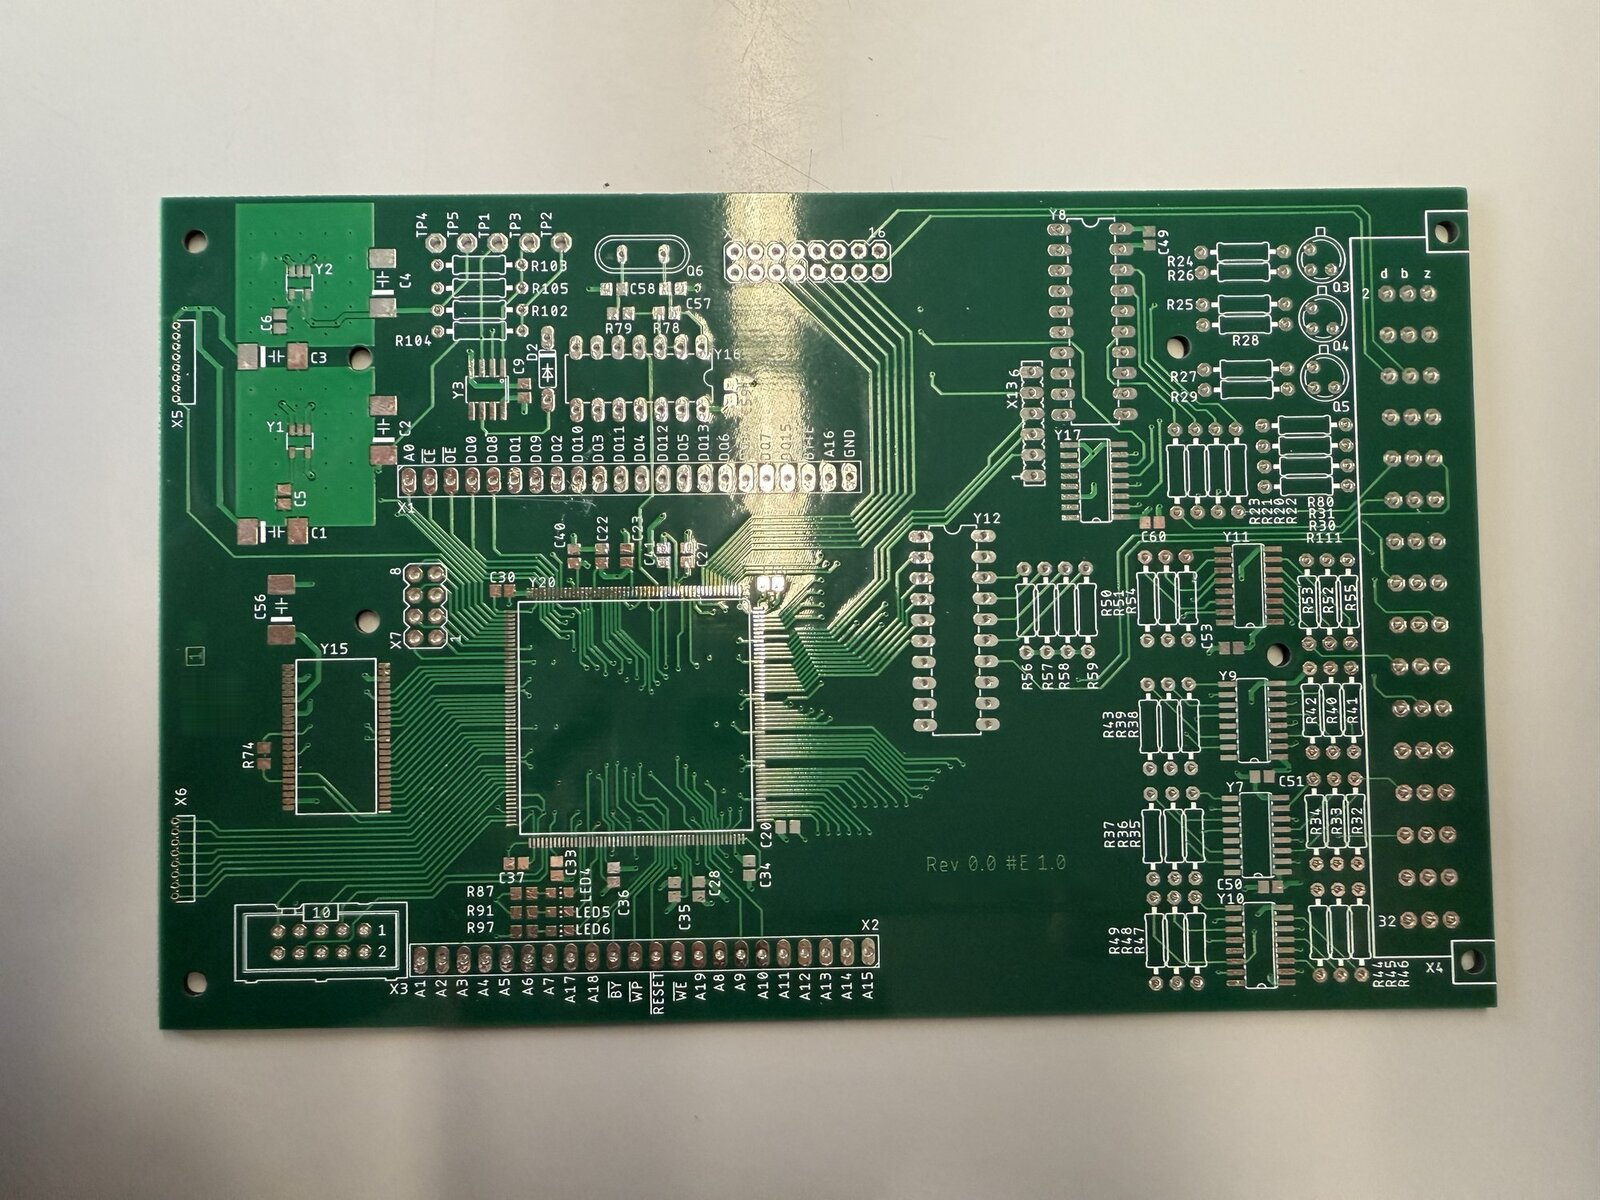
\includegraphics[width=0.75\textwidth]{photos/base_board_bare_top.jpg}
	\caption[Bare Base Board]{Base Board, unpopulated (top view). The silkscreen reads Rev~0.0: the Base Board was reused in its inherited revision (\Cref{sec:pcb_design_impl}).}
	\label{fig:bare_base_board}
\end{figure}

\begin{figure}[H]
	\centering
	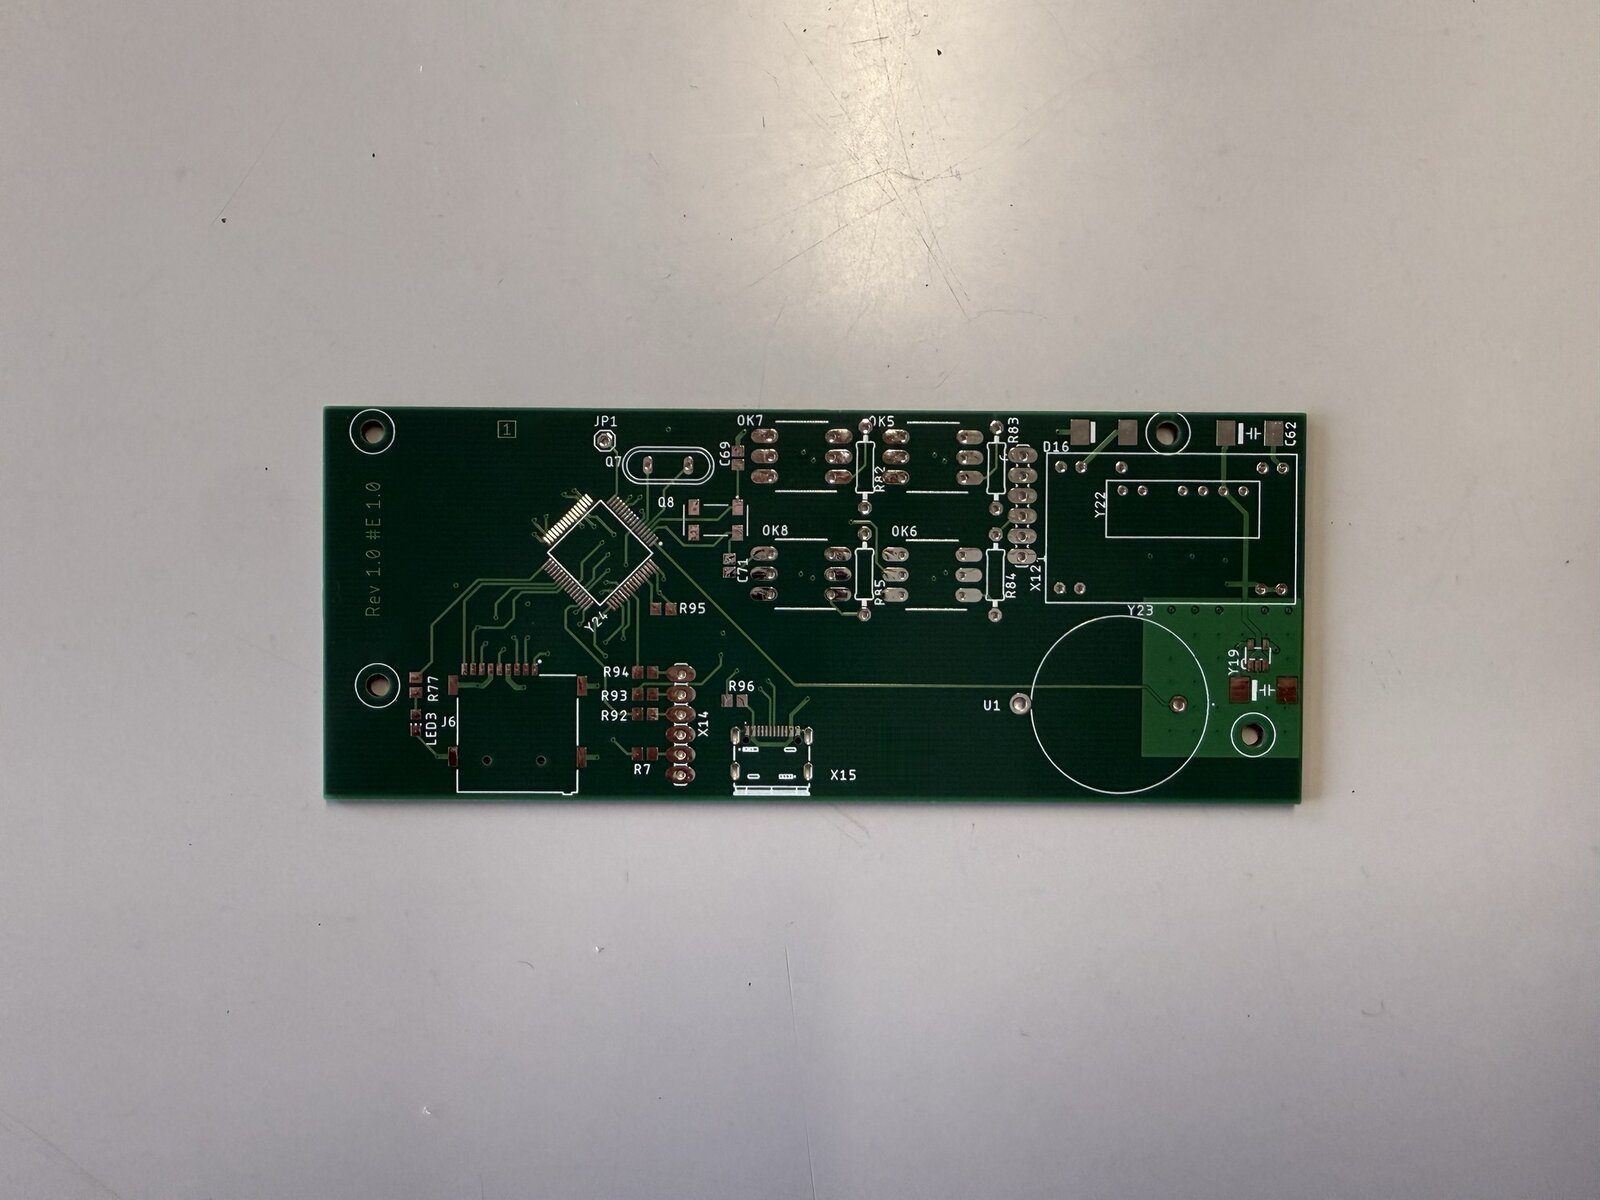
\includegraphics[width=0.75\textwidth]{photos/rev1_stm32_board_bare_top.jpg}
	\caption[Rev 1.0 Bare STM32 Board]{Corrected Rev~1.0 \gls{stm32} Diagnostics Board, unpopulated (top view), with the SWD header \texttt{X14} and its series resistors \texttt{R7} and \texttt{R92}--\texttt{R94}.}
	\label{fig:rev1_bare_stm32_board}
\end{figure}


% ------------------------------------------------------------
\section{Schematic}
\label{sec:app_schematic_sheets}

The schematic of all four boards is one Eagle project of four sheets, organised by function rather than by board. \Cref{tab:bom} lists which board carries each part.

\begin{figure}[H]
	\centering
	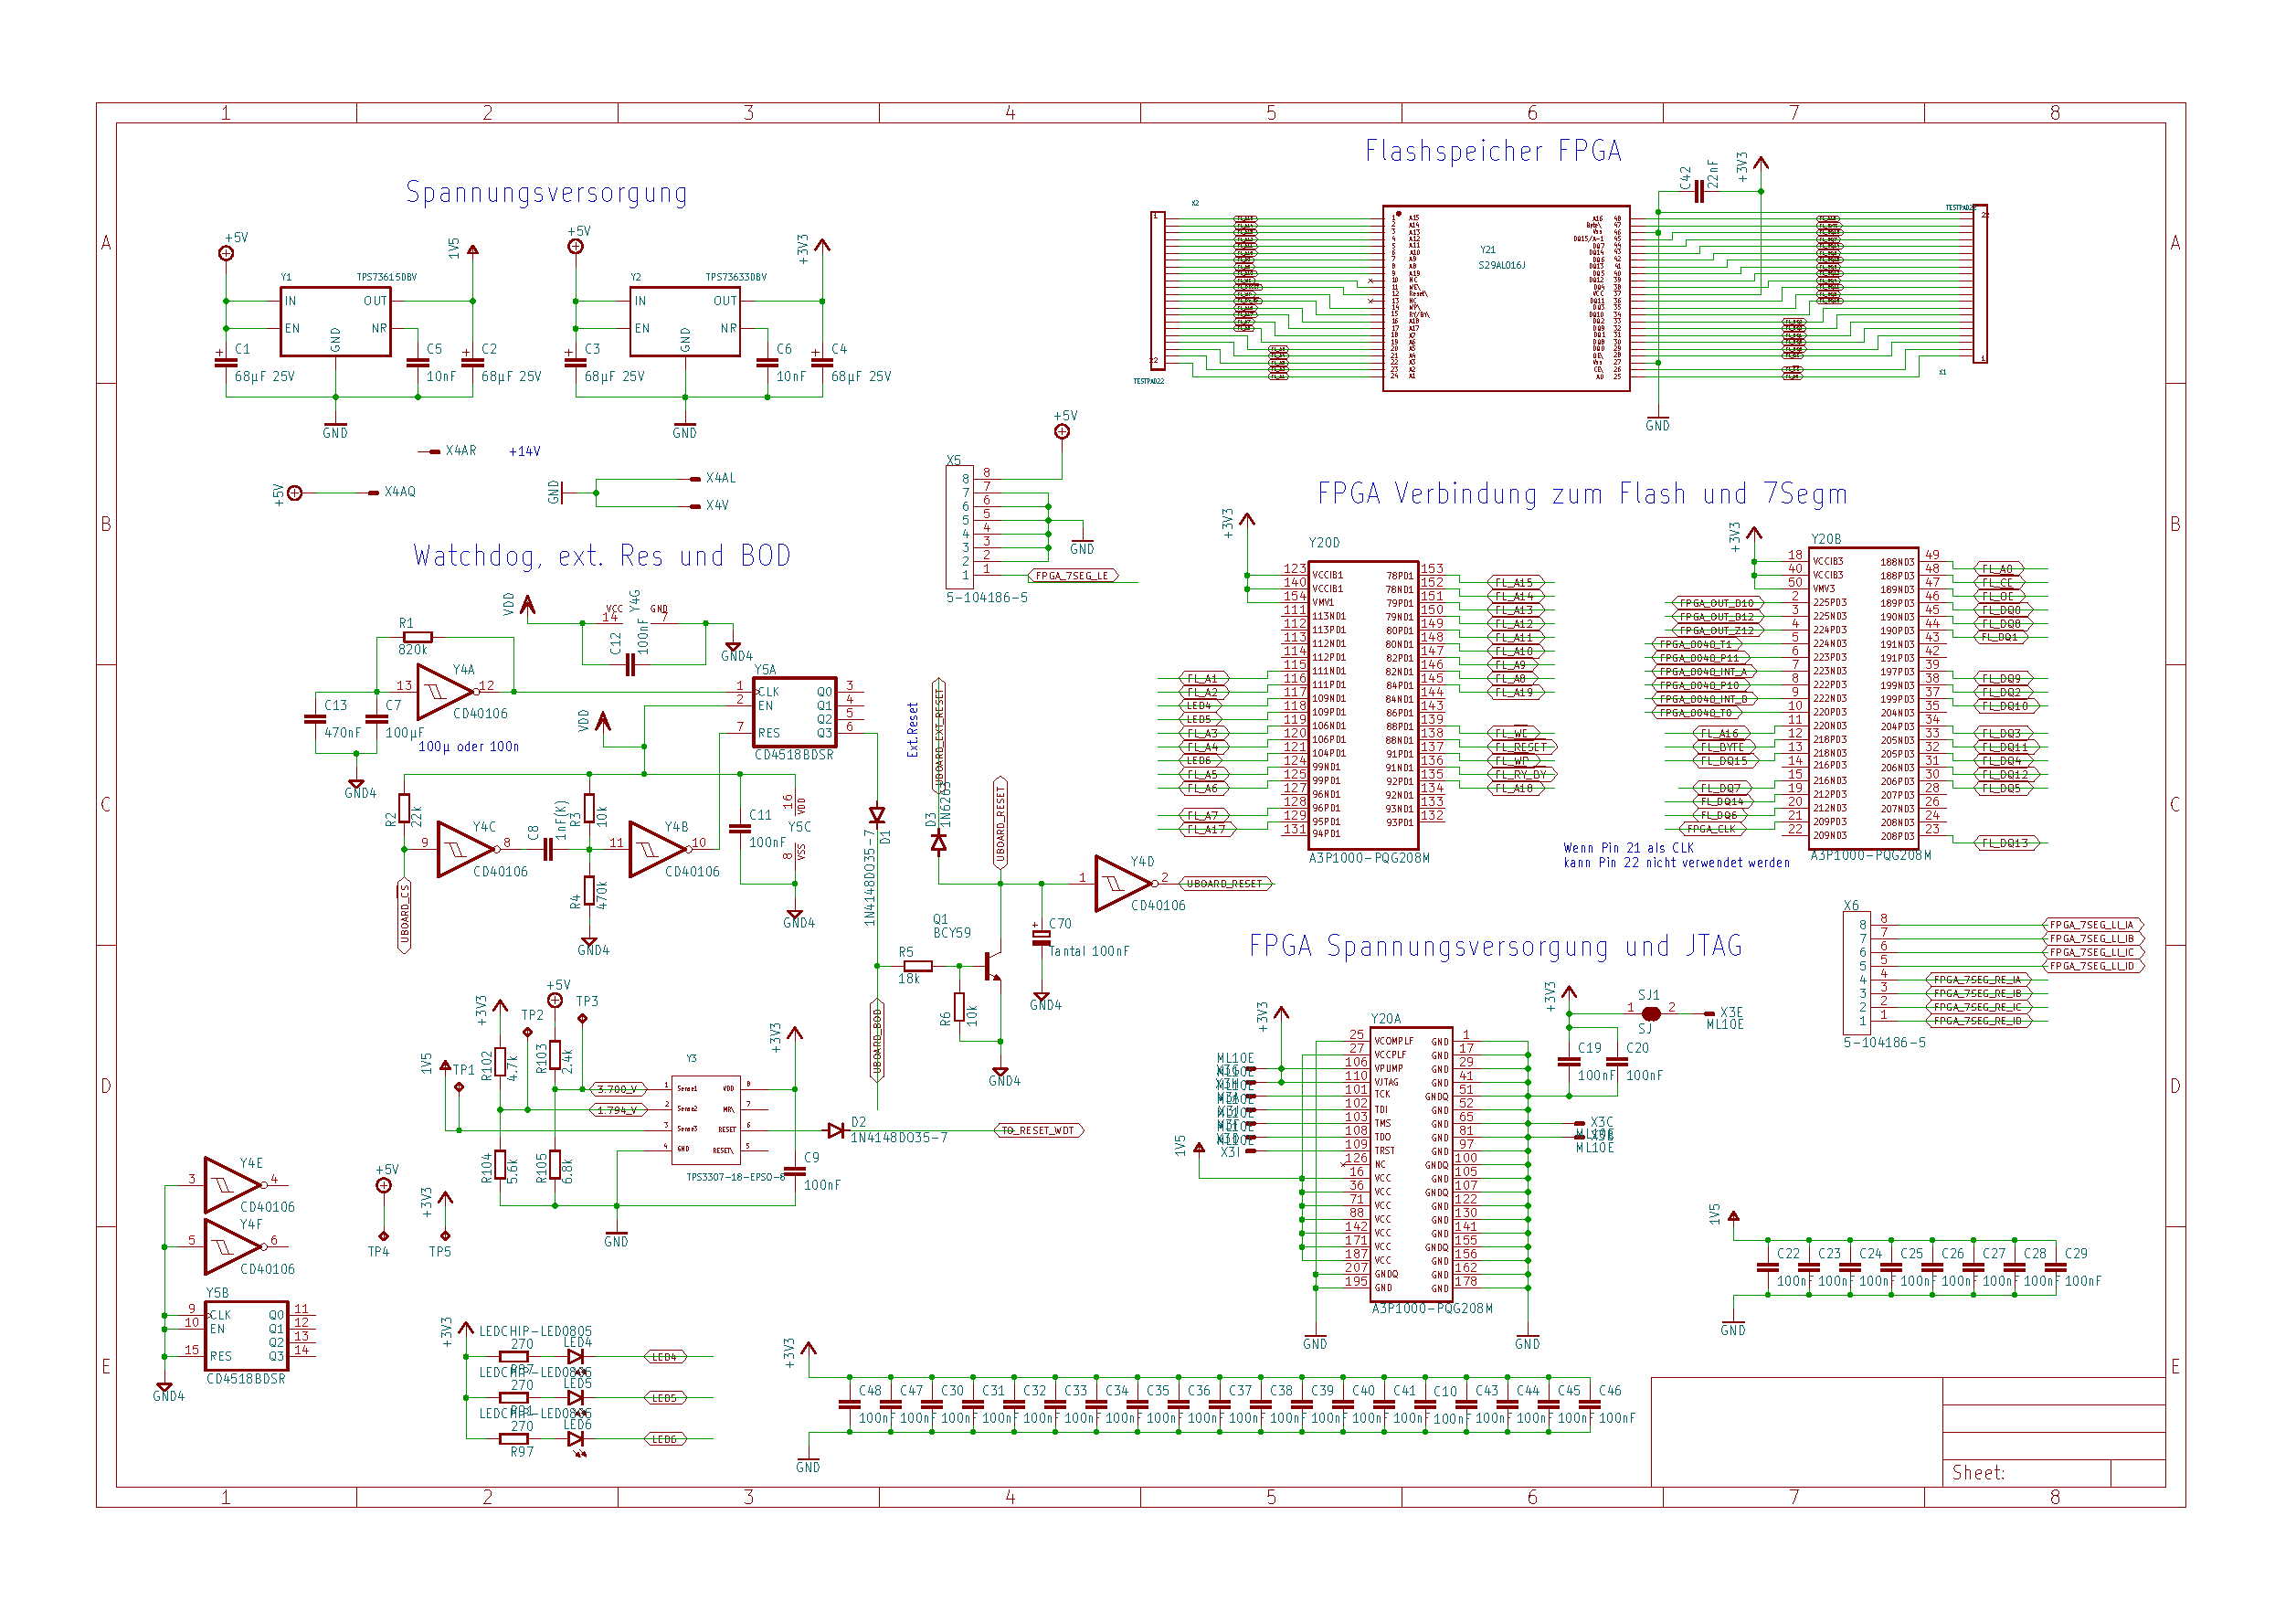
\includegraphics[trim=48 52 55 52, clip, width=0.85\textheight, angle=90]{schematic/sheet1.pdf}
	\caption[Schematic Sheet 1]{Schematic sheet~1: power supply (\texttt{Y1}, \texttt{Y2}), external watchdog with reset and brown-out detection (\texttt{Y3}--\texttt{Y5}, \texttt{Q1}), Flash~\gls{rom} (\texttt{Y21}) with its test fields \texttt{X1}/\texttt{X2}, \gls{fpga} supply and \gls{jtag} header \texttt{X3}. Rendered with KiCad from the Eagle design file of 2024. Design: Leyer~\cite{leyer2023}.}
	\label{fig:schematic_sheet1}
\end{figure}

\begin{figure}[H]
	\centering
	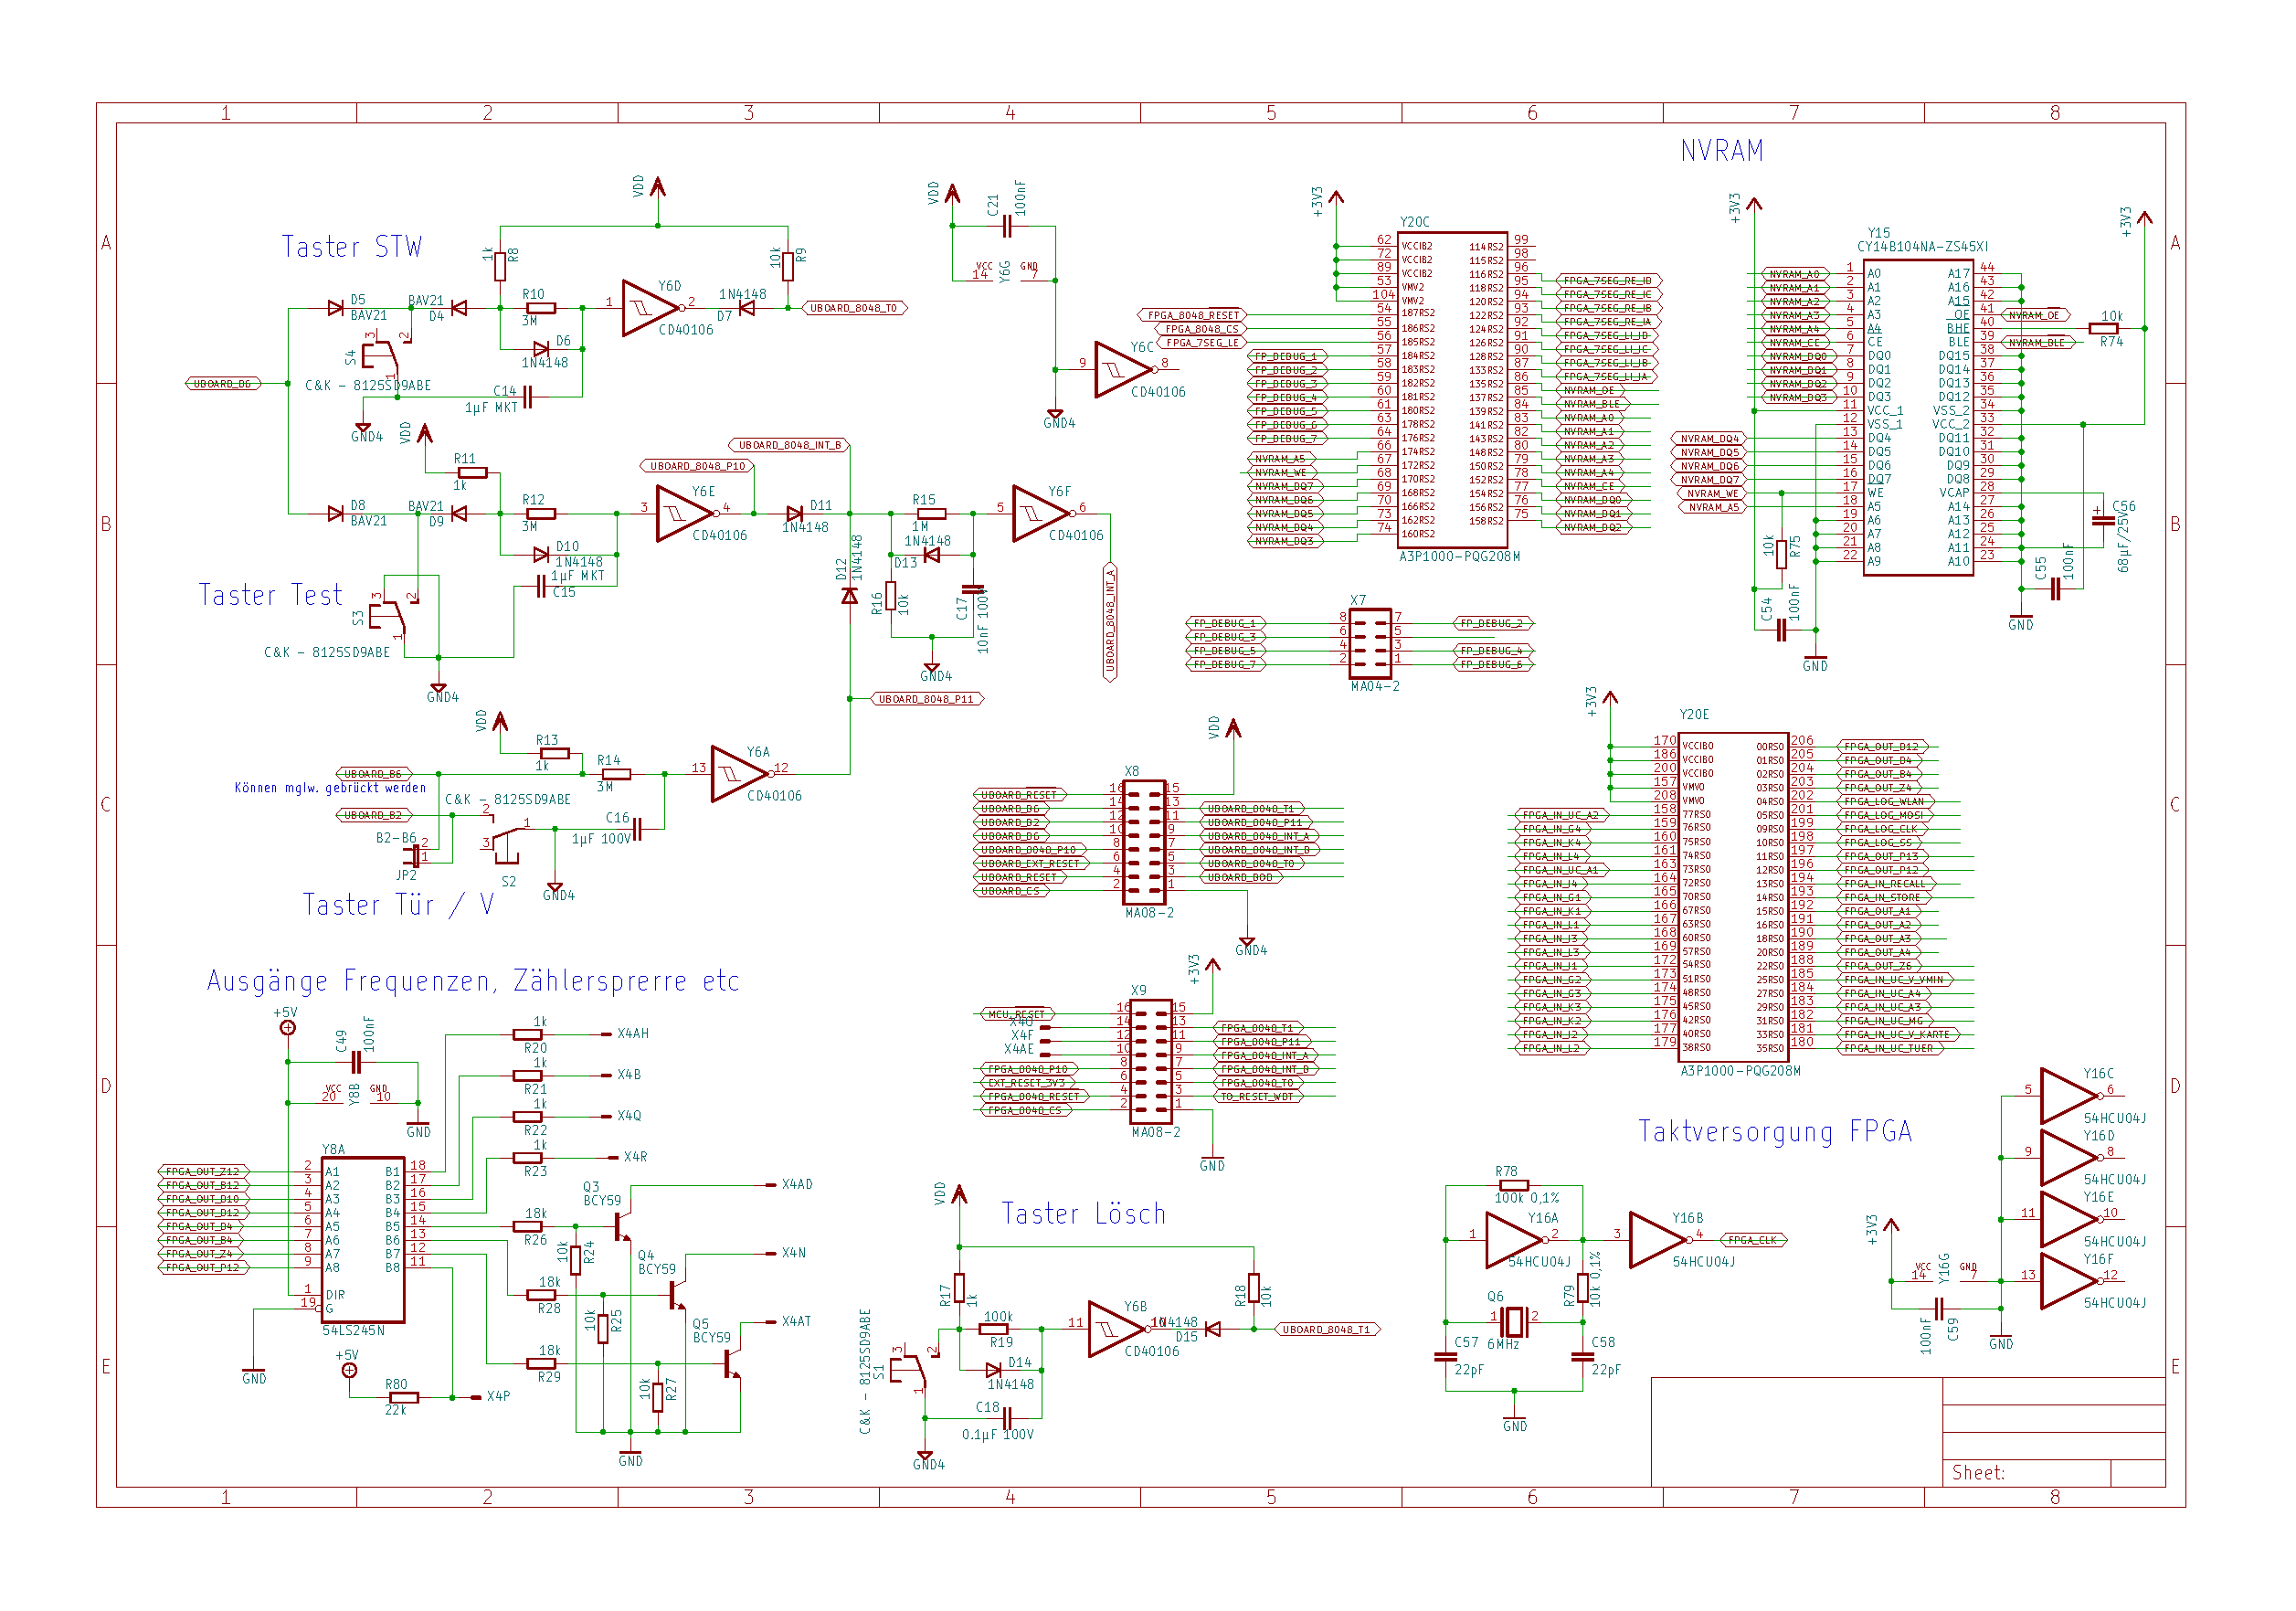
\includegraphics[trim=48 52 55 52, clip, width=0.85\textheight, angle=90]{schematic/sheet2.pdf}
	\caption[Schematic Sheet 2]{Schematic sheet~2: operator buttons with debouncing (\texttt{S1}--\texttt{S4}, \texttt{Y6}), output drivers (\texttt{Y8}, \texttt{Q3}--\texttt{Q5}), \gls{nvram} (\texttt{Y15}), \SI{6}{\mega\hertz} clock (\texttt{Y16}, \texttt{Q6}), the headers \texttt{X8} and \texttt{X9} of the ribbon cable between the Upper Board and the Base Board, and the \gls{fpga} debug header \texttt{X7}. Rendered with KiCad from the Eagle design file of 2024. Design: Leyer~\cite{leyer2023}.}
	\label{fig:schematic_sheet2}
\end{figure}

\begin{figure}[H]
	\centering
	% slightly smaller than the other sheets, so that the note on defect B6 fits below the caption
	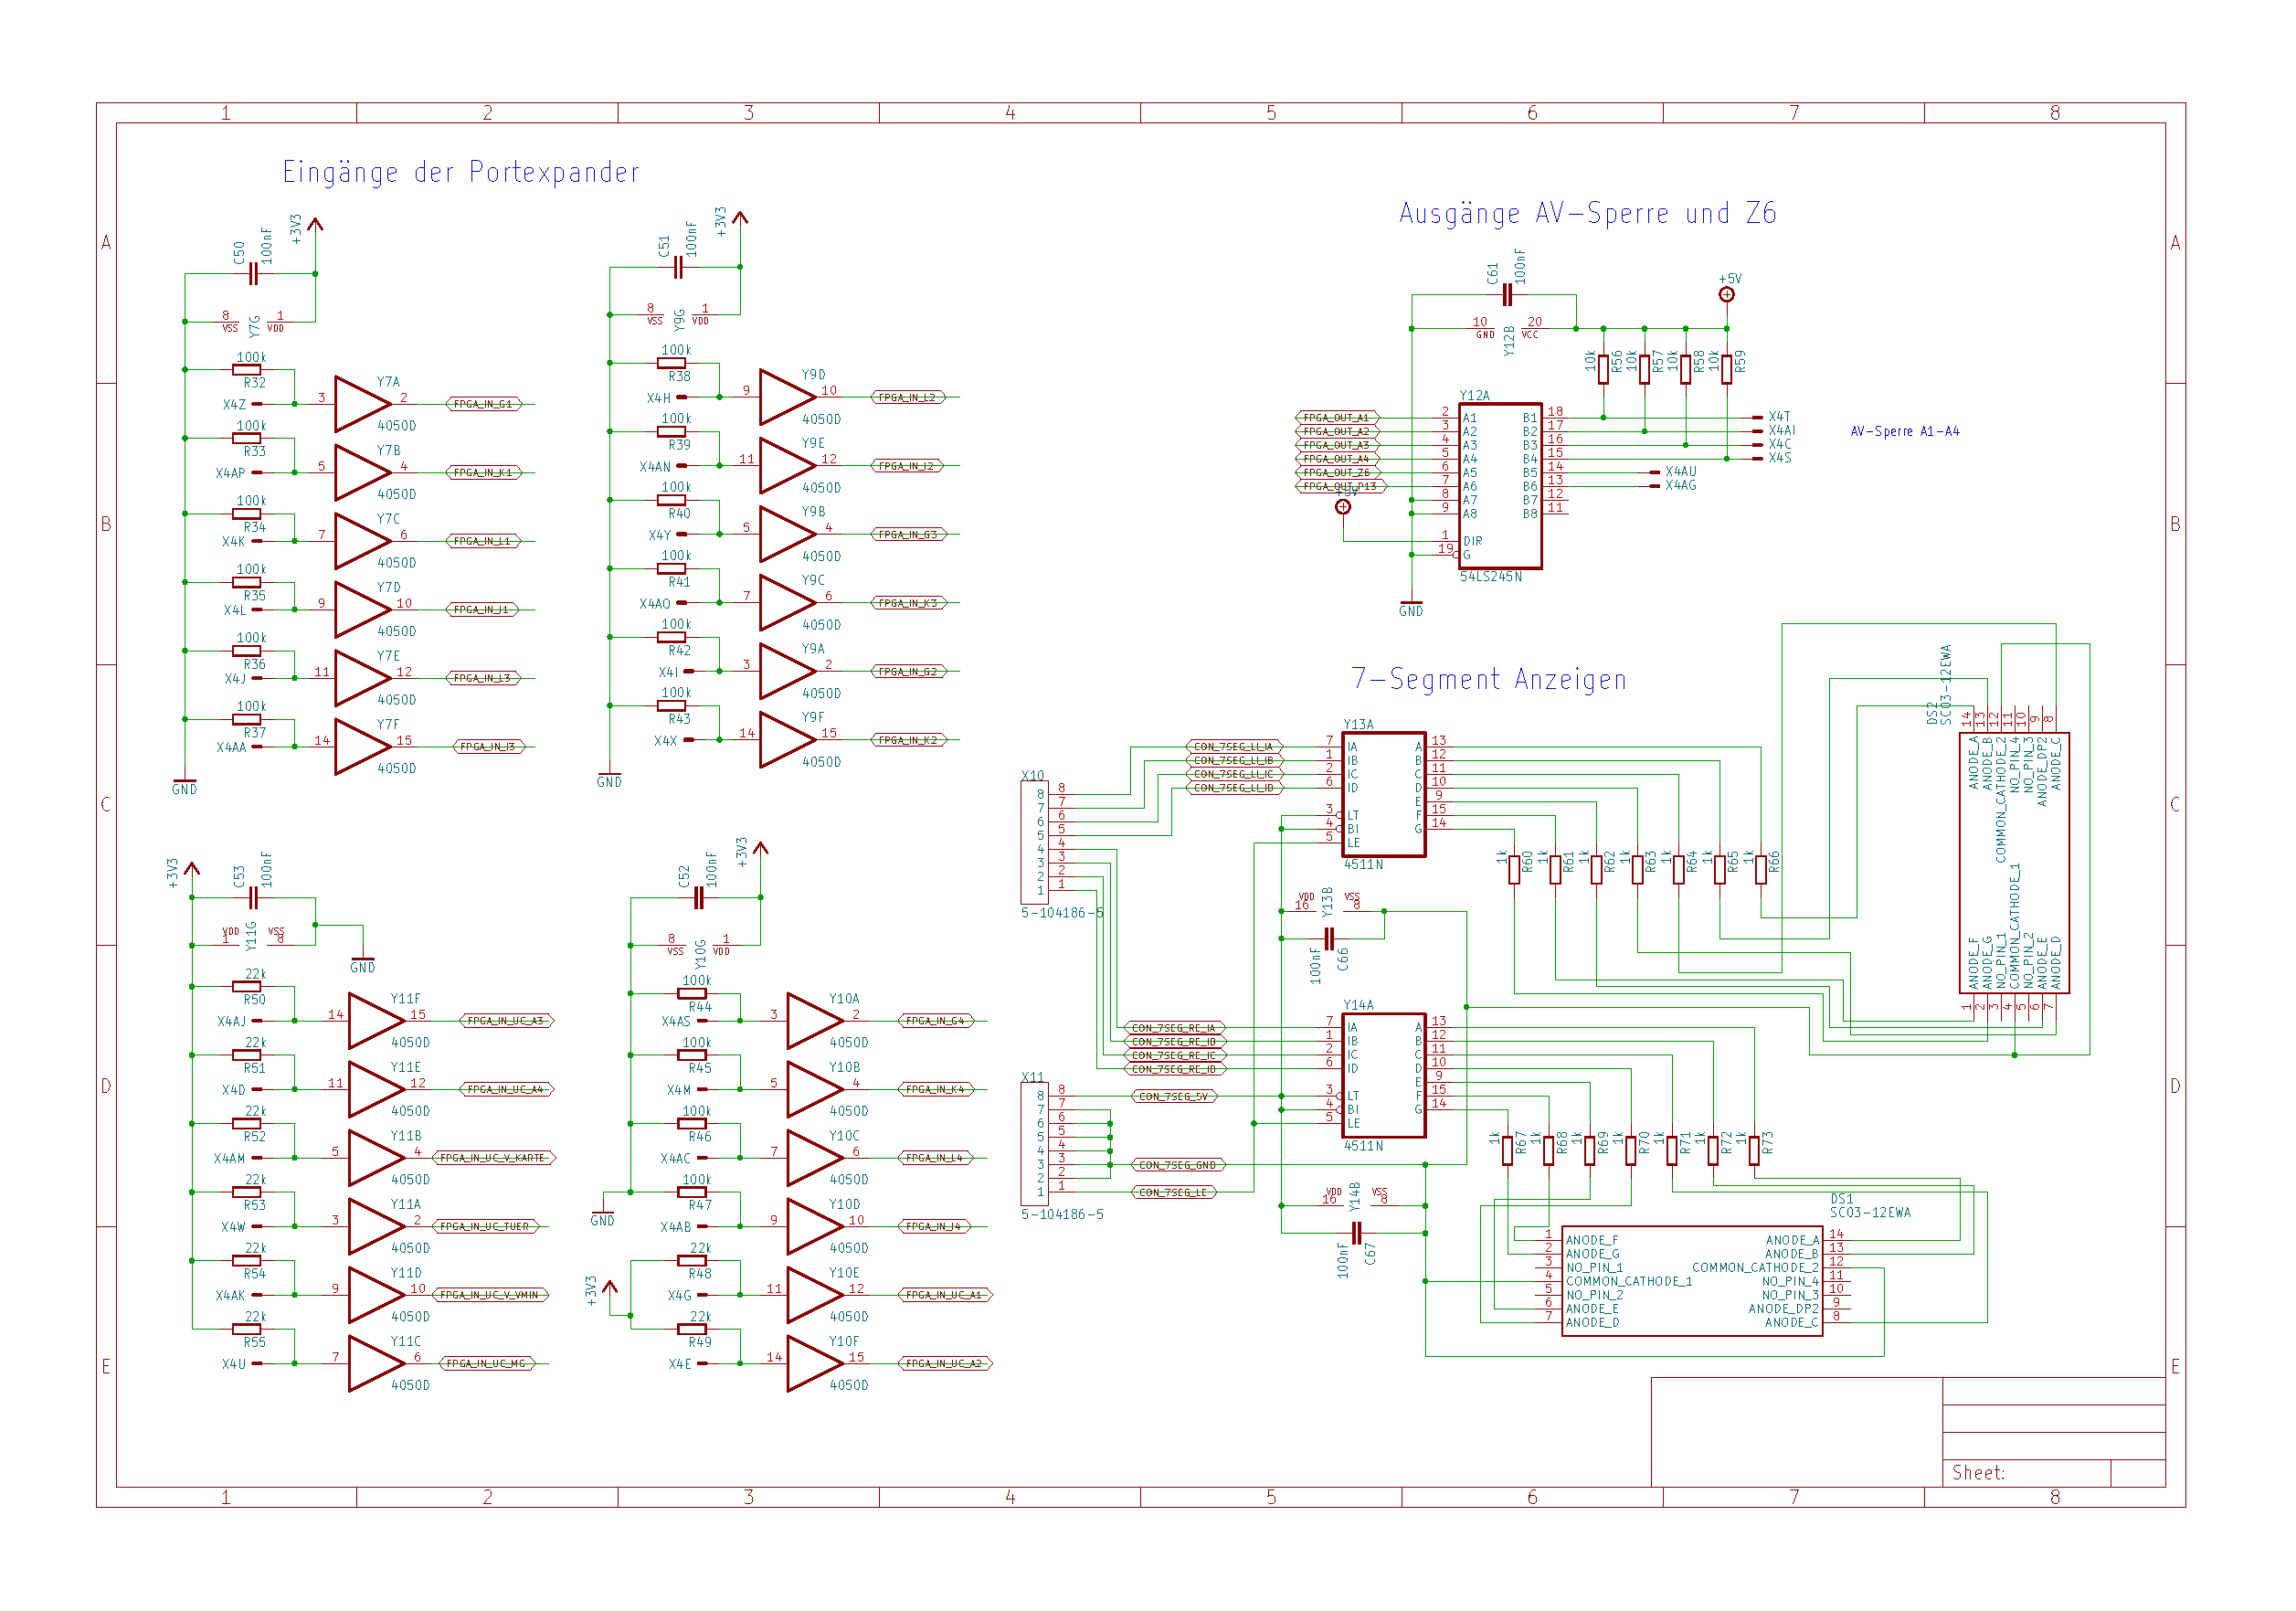
\includegraphics[trim=48 52 55 52, clip, width=0.8\textheight, angle=90]{schematic/sheet3.pdf}
	\caption[Schematic Sheet 3]{Schematic sheet~3: input level shifters for the system connector \texttt{X4} (\texttt{Y7}, \texttt{Y9}--\texttt{Y11}), output drivers (\texttt{Y12}) and the 7-segment display board with its drivers (\texttt{Y13}, \texttt{Y14}) and the \texttt{SC03-12EWA} displays \texttt{DS1} and \texttt{DS2}, with which this work replaced the end-of-life \texttt{5082-7613} displays. Rendered with KiCad from the Eagle design file of 2024. Design: Leyer~\cite{leyer2023}.}
	\label{fig:schematic_sheet3}

	\smallskip
	\begin{minipage}{\textwidth}
		\footnotesize
		Note: The driver-to-display assignment drawn on this sheet, \texttt{Y13} (left digit) to \texttt{DS2} and \texttt{Y14} (right digit) to \texttt{DS1}, is reversed against the design files of 2023, in which \texttt{Y13} drives the display at the position of \texttt{DS1}; it produced defect B6 (\Cref{tab:bug_taxonomy}), which the follow-on team worked around in \texttt{atop.vhd}~\cite[p.~13]{savchuk2025}. The corrected \texttt{atop.vhd} is not archived.
	\end{minipage}
\end{figure}

\begin{figure}[H]
	\centering
	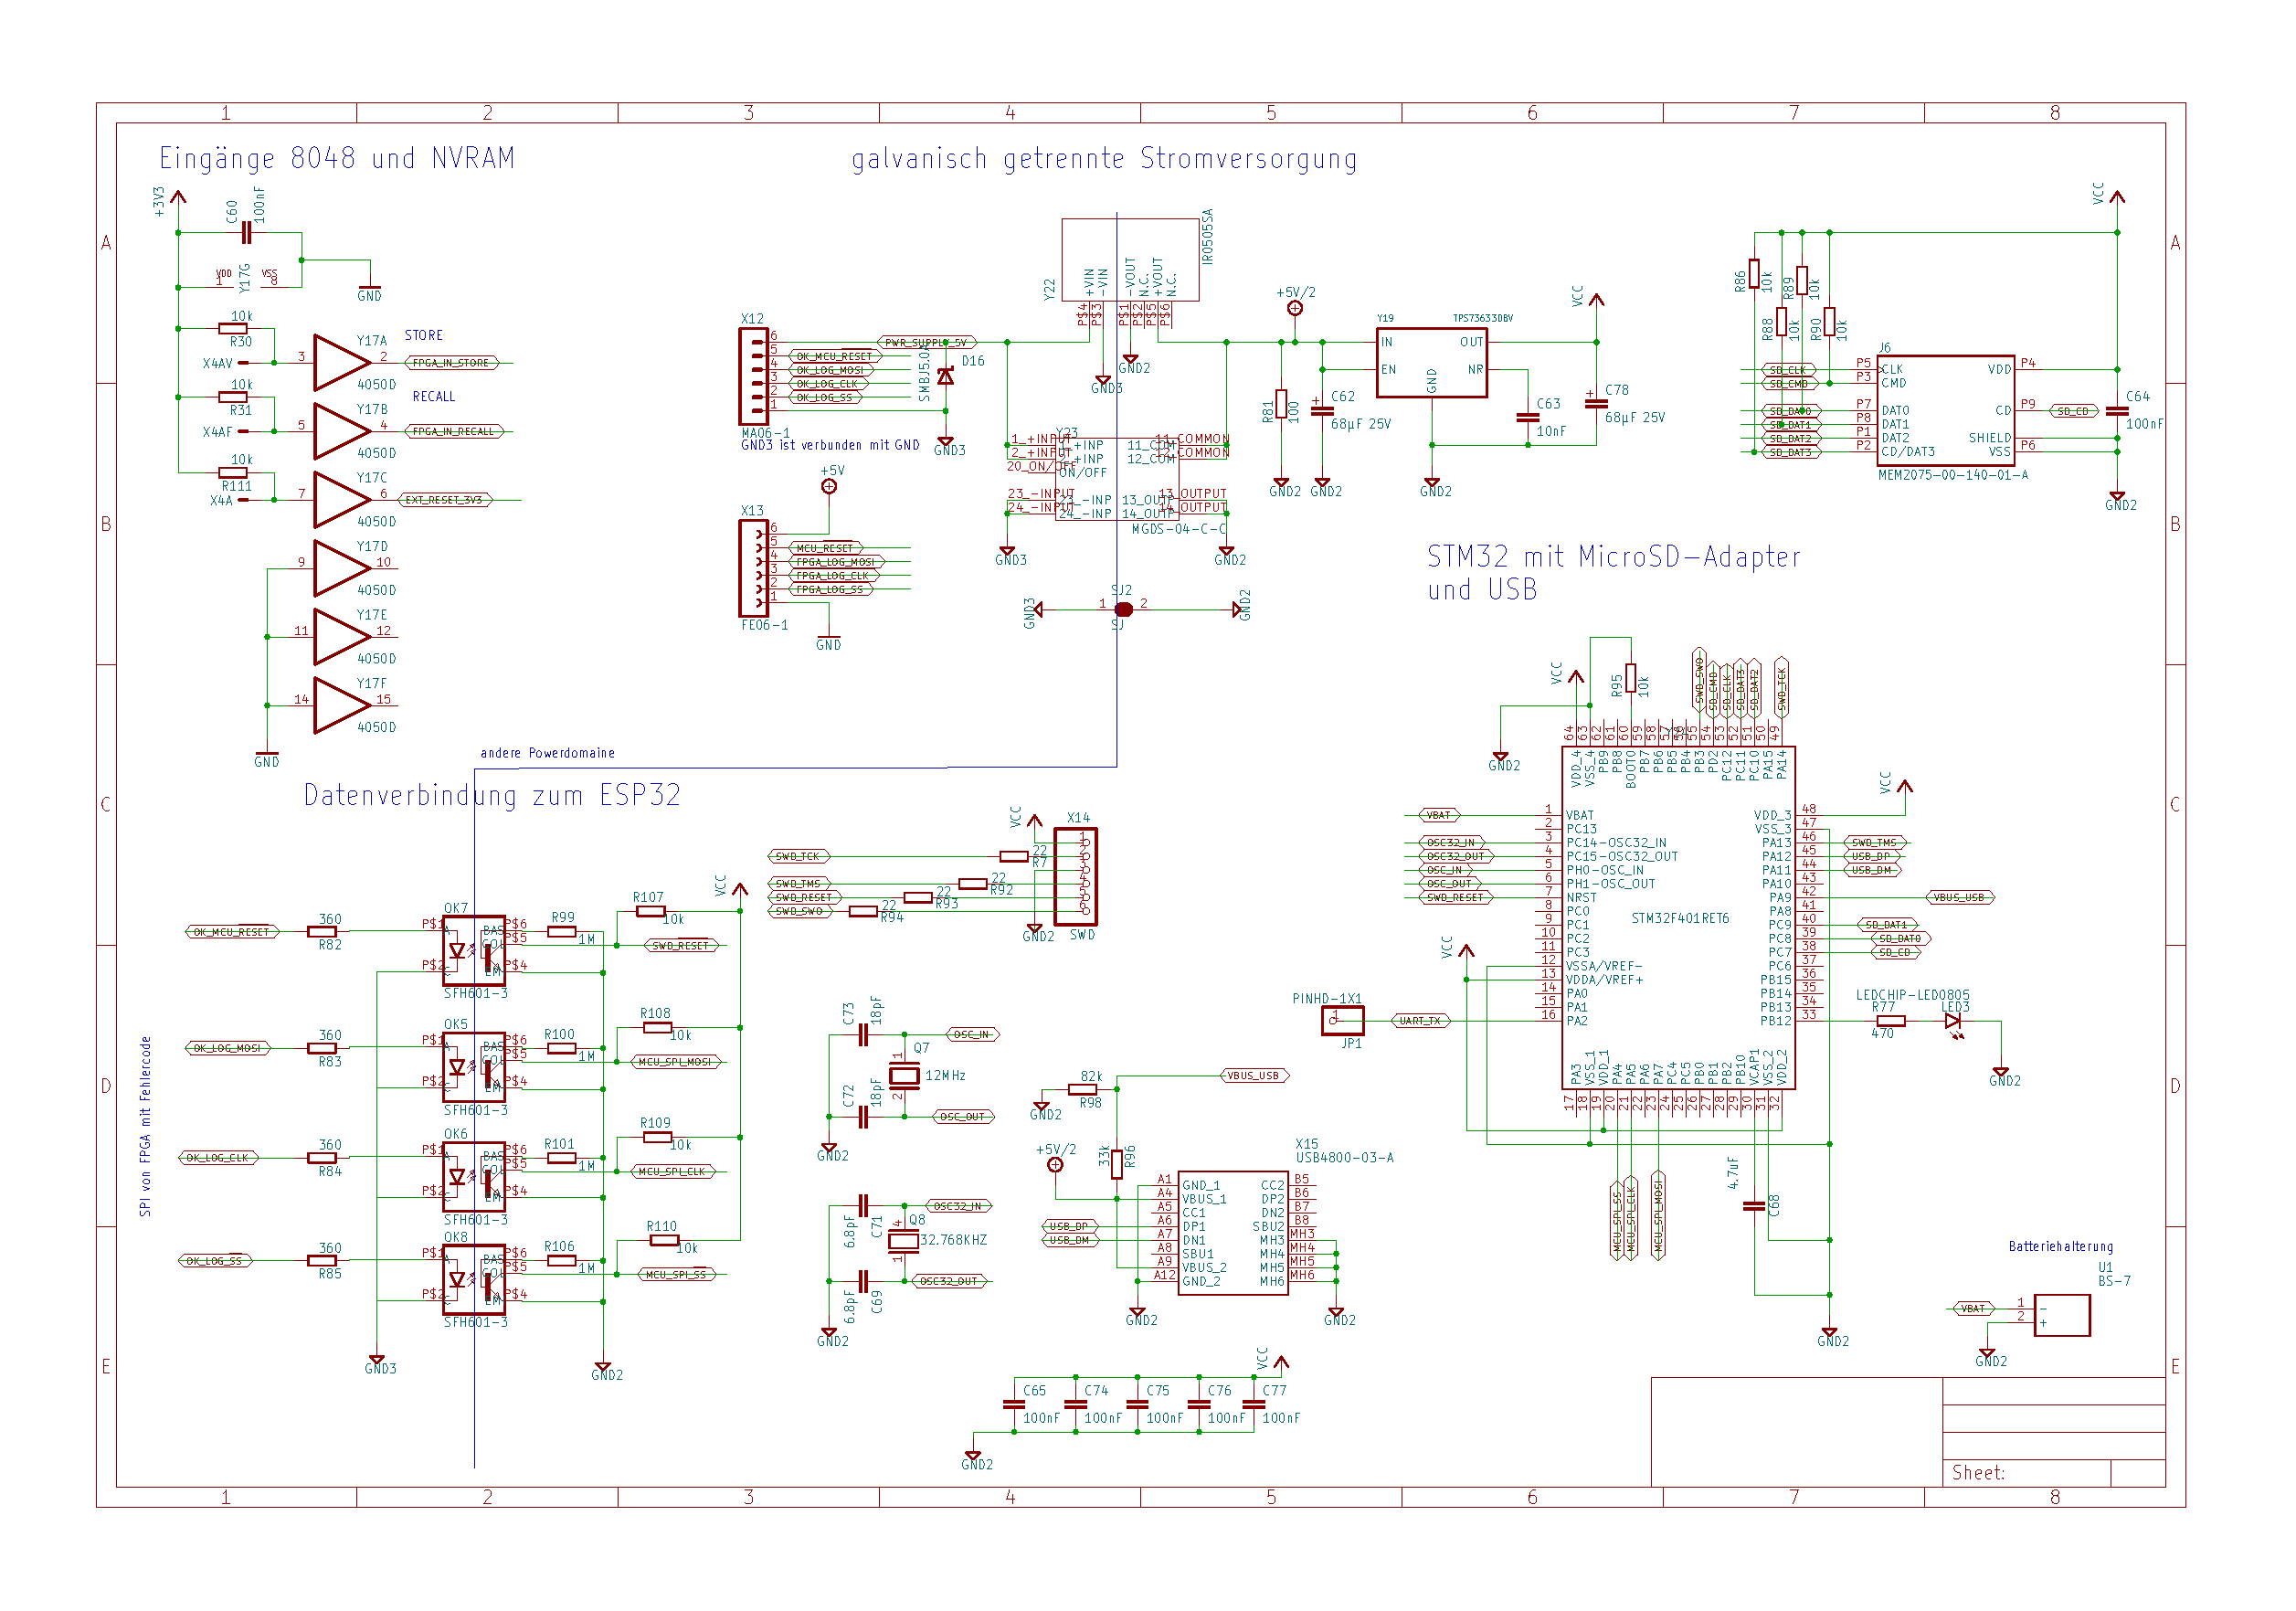
\includegraphics[trim=48 52 55 52, clip, width=0.85\textheight, angle=90]{schematic/sheet4.pdf}
	\caption[Schematic Sheet 4]{Schematic sheet~4: \gls{stm32} Diagnostics Board with isolated supply (\texttt{Y19}, \texttt{Y22}, \texttt{Y23}), optocoupled link (\texttt{OK5}--\texttt{OK8}), MicroSD socket (\texttt{J6}), \gls{usb} Type-C connector (\texttt{X15}), SWD header (\texttt{X14}) and \gls{rtc} crystal (\texttt{Q8}); the block \enquote{Eingänge 8048 und NVRAM} (inputs of the 8048 and the~\gls{nvram}) holds the Base Board input buffer \texttt{Y17}. The label \enquote{Datenverbindung zum ESP32} is left over from an earlier variant based on an ESP32 module. Rendered with KiCad from the Eagle design file of 2024. Design: Leyer~\cite{leyer2023}.}
	\label{fig:schematic_sheet4}
\end{figure}

\clearpage

% ------------------------------------------------------------
\section{Base Board (Unterplatine) Layout}
\label{sec:app_base_board_schematics}

\begin{figure}[H]
	\centering
	\includegraphicsowngroup[width=0.9\textwidth]{layout/top/unterplatine.pdf}
	\caption[Base Board Layout (Top)]{Base Board (Rev~0.0) PCB layout, top view, showing the component placement. Rendered with KiCad from the Eagle design file of 2024, without the third-party logo and board designation. Design: Leyer~\cite{leyer2023}.}
	\label{fig:base_layout_top}
\end{figure}

\begin{figure}[H]
	\centering
	\includegraphicsowngroup[width=0.9\textwidth]{layout/bottom/unterplatine.pdf}
	\caption[Base Board Layout (Bottom)]{Base Board (Rev~0.0) PCB layout, bottom view (mirrored). Rendered with KiCad from the Eagle design file of 2024, without the third-party logo. Design: Leyer~\cite{leyer2023}.}
	\label{fig:base_layout_bottom}
\end{figure}

\clearpage

% ------------------------------------------------------------
\section[Upper Board (Oberplatine) and LED Board Layouts]{Upper Board (Oberplatine) and LED Board\\Layouts}
\label{sec:app_upper_board_schematics}

\begin{figure}[H]
	\centering
	\includegraphicsowngroup[width=0.9\textwidth]{layout/top/oberplatine.pdf}
	\caption[Upper Board Layout (Top)]{Upper Board (Rev~1.0) PCB layout, top view. Rendered with KiCad from the Eagle design file of 2024, without the third-party logo and board designation. Design: Leyer~\cite{leyer2023}.}
	\label{fig:upper_layout_top}
\end{figure}

\begin{figure}[H]
	\centering
	\includegraphicsowngroup[width=0.9\textwidth]{layout/bottom/oberplatine.pdf}
	\caption[Upper Board Layout (Bottom)]{Upper Board (Rev~1.0) PCB layout, bottom view (mirrored). Rendered with KiCad from the Eagle design file of 2024, without the third-party logo. Design: Leyer~\cite{leyer2023}.}
	\label{fig:upper_layout_bottom}
\end{figure}

\phantomsection
\label{sec:app_led_board_schematics}
\begin{figure}[H]
	\centering
	\includegraphicsowngroup[width=0.9\textwidth]{layout/top/led.pdf}
	\caption[LED Board Layout (Top)]{LED Board (Rev~1.0) PCB layout, top view. Rendered with KiCad from the Eagle design file of 2024, without the third-party logo and board designation. Design: Leyer~\cite{leyer2023}.}
	\label{fig:led_layout_top}
\end{figure}

\begin{figure}[H]
	\centering
	\includegraphicsowngroup[width=0.9\textwidth]{layout/bottom/led.pdf}
	\caption[LED Board Layout (Bottom)]{LED Board (Rev~1.0) PCB layout, bottom view (mirrored), with the \texttt{SC03-12EWA} displays \texttt{DS1} and \texttt{DS2}. Rendered with KiCad from the Eagle design file of 2024. Design: Leyer~\cite{leyer2023}.}
	\label{fig:led_layout_bottom}
\end{figure}


% ------------------------------------------------------------
\section{STM32 Diagnostics Board Layout}
\label{sec:app_stm32_board_schematics}

\begin{figure}[H]
	\centering
	\includegraphicsowngroup[width=0.9\textwidth]{layout/top/stm32.pdf}
	\caption[STM32 Board Layout (Top)]{\gls{stm32} Diagnostics Board (Rev~1.0) PCB layout, top view. Rendered with KiCad from the Eagle design file of 2024, without the third-party logo and board designation. Design: Leyer~\cite{leyer2023}.}
	\label{fig:stm32_layout_top}
\end{figure}

\begin{figure}[H]
	\centering
	\includegraphicsowngroup[width=0.9\textwidth]{layout/bottom/stm32.pdf}
	\caption[STM32 Board Layout (Bottom)]{\gls{stm32} Diagnostics Board (Rev~1.0) PCB layout, bottom view (mirrored). Rendered with KiCad from the Eagle design file of 2024, without the third-party logo. Design: Leyer~\cite{leyer2023}.}
	\label{fig:stm32_layout_bottom}
\end{figure}


% ------------------------------------------------------------
\section{Connectors}
\label{sec:app_connectors}
The boards are connected by standard pin headers and sockets. The Base Board carries the LED Board on two TE AMPMODU System~50 headers (\texttt{X5}/\texttt{X6} mating with \texttt{X10}/\texttt{X11})~\cite{te_ampmodu_sys50} and the \gls{stm32} Diagnostics Board on a six-pin header pair (\texttt{X13}/\texttt{X12}); the Upper Board is connected by a ribbon cable between the 2$\times$8 headers \texttt{X9} and \texttt{X8}. The vehicle side is reached through the 48-pin DIN~41612 type~F system connector \texttt{X4}.

% back to the page layout of the other chapters
\flushbottom
